\chapter{INTRODUCTION}\label{chp:LABEL_CHP_1}


Computer graphics is a field of computer science focused on the generation, manipulation, and display of digital images. Since its inception, it has transformed various industries such as entertainment, architecture, and design, enabling the creation of virtual worlds and realistic environments. As machine processing increases and researchers constantly push the boundaries of technology, increasingly complex and detailed graphics have been made possible.


With advancements in rendering techniques and algorithms, methods such as Ray Tracing and Path Tracing [REFERENCIA] have emerged to accurately simulate the behavior of light, textures, and materials in three-dimensional environments. These methods are widely used in still images and animations, though they require significant computational power. Additionally, technologies like shaders \footnote{https://www.khronos.org/opengl/wiki/shader}, which allow customization at the pixel level, have become essential in gaming and simulation environments, delivering increasingly immersive visual experiences to users.


In this context, Ray Marching stands out as an innovative technique, particularly for real-time rendering of complex surfaces and fractals. Unlike traditional Ray Tracing, Ray Marching uses an iterative approach to detect surfaces within a Signed Distance Field (SDF) [REFERENCIA]. An SDF stores the shortest distance from any point in space to the closest surface, which allows it to describe smooth and detailed shapes, without needing traditional polygonal geometry. This technique is especially useful for rendering scenes involving implicit geometry, such as fractals and abstract scenarios, and is frequently applied in virtual reality environments and visual effects for games.


\begin{figure}[ht]
    \centering
    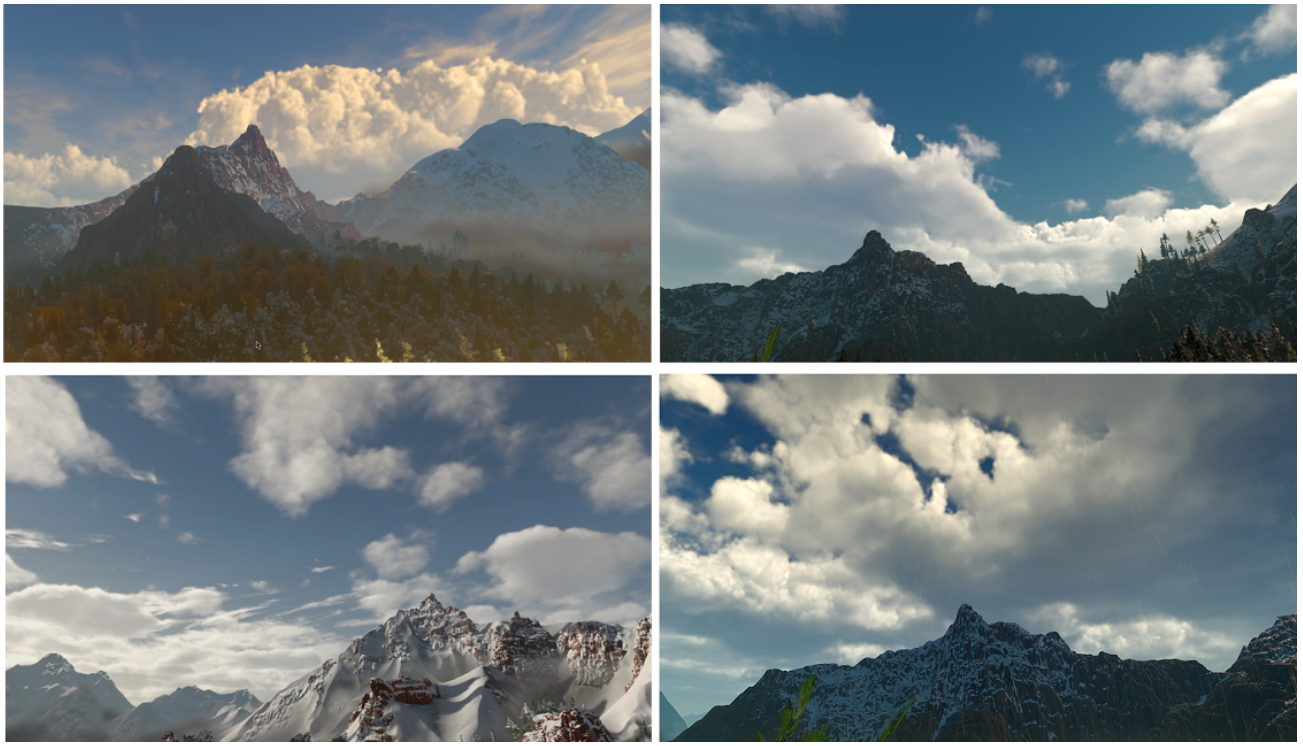
\includegraphics[width=13.83cm,height=9.1cm]{imagens/raymarched-clouds-schneider.png} 
    \caption{Raymarched Clouds obtained by Schneider et al.\protect\footnotemark}
    \label{fig:internet}
\end{figure}
\footnotetext{Source: Schneider et al.}

Ray Marching has found several practical applications in the gaming industry, particularly for rendering complex and dynamic scenes. In the Frostbite Engine [REFERENCIA], used in titles such as Battlefield V, Ray Marching is employed to render highly realistic volumetric clouds. This approach allows the engine to simulate depth, light scattering, and other atmospheric effects in real time, creating lifelike skies that respond dynamically to environmental lighting conditions. 

\footnotetext{Source: https://media.contentapi.ea.com/content/dam/eacom/frostbite/files/s2016-pbs-frostbite-sky-clouds-new.pdf}

\section{Scope and Objective}

In this document, we explore Ray Marching as implemented in GLSL and compare its strengths to traditional ray tracing methods. Our primary objective is to demonstrate Ray Marching's unique capabilities, particularly its use of SDFs, which allow for precise control over shapes and blending effects that are challenging to achieve with ray tracing.


We also explore the potential of Ray Marching for procedural rendering, showcasing its use in creating complex noise patterns and highly realistic volumetric effects, including cloud rendering. By examining these features, we aim to highlight Ray Marching’s versatility and its advantages in generating intricate, dynamic visuals for real-time applications.

\section{Methodology}

We take an iterative approach to explore the Ray Marching algorithm, showcasing its capacity to render smooth, noisy, and dynamic surfaces. Real-time 3D applications often rely on graphics APIs such as OpenGL, DirectX, or Vulkan for GPU programming. To simplify development and focus on Ray Marching itself, we use Shadertoy — a tool for running fragment shaders written in GLSL (OpenGL Shading Language) without the extensive setup. Fragment shaders are GPU programs that process each pixel on the screen, taking inputs such as the pixel position and canvas resolution.

\section{Text Structure}

O que cada capítulo fala. (pra depois)